\section{Discussion}
\begin{figure}[h]
    \centering
    \begin{tabular}{cc}
        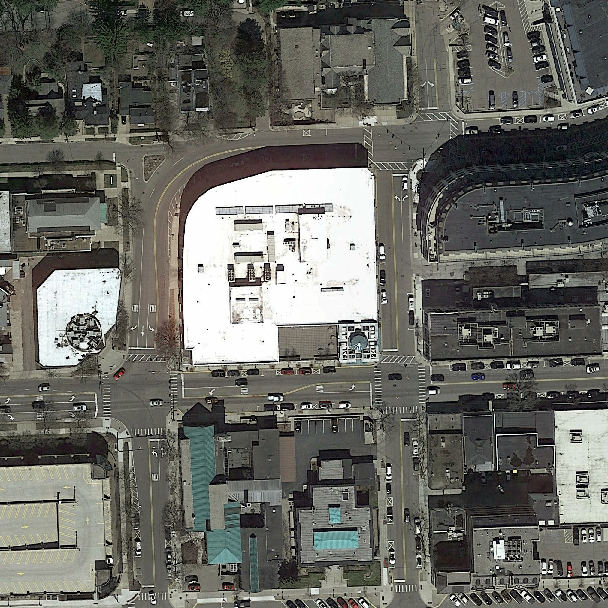
\includegraphics[width=0.4\linewidth]{original.png} & 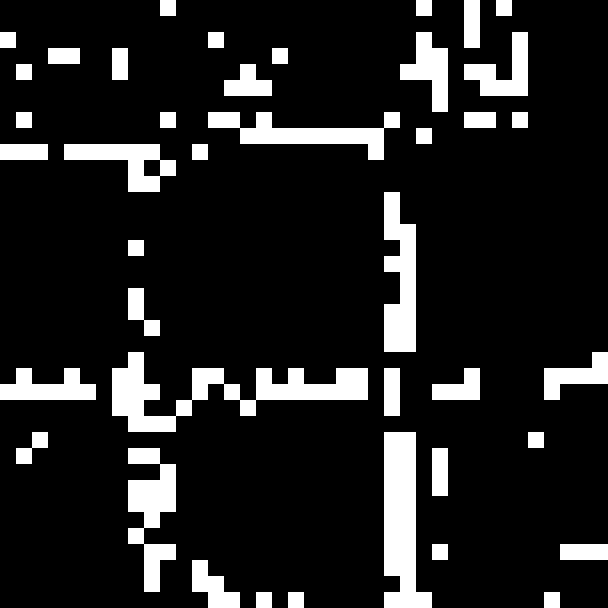
\includegraphics[width=0.4\linewidth]{baseline.png} \\
        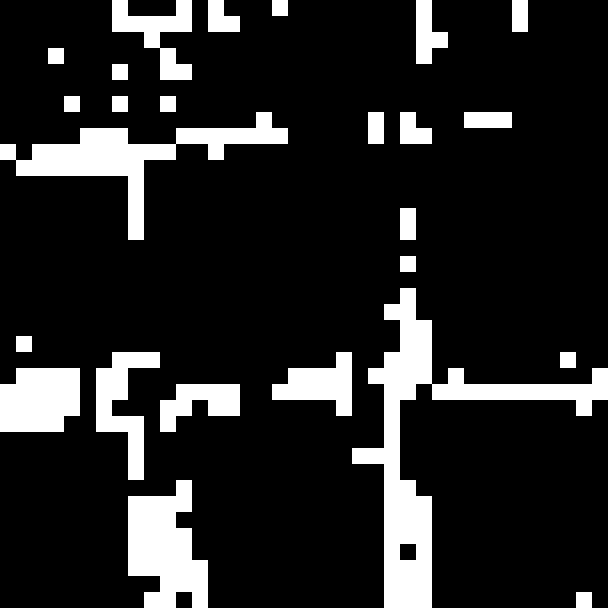
\includegraphics[width=0.4\linewidth]{baselinepp.png} & 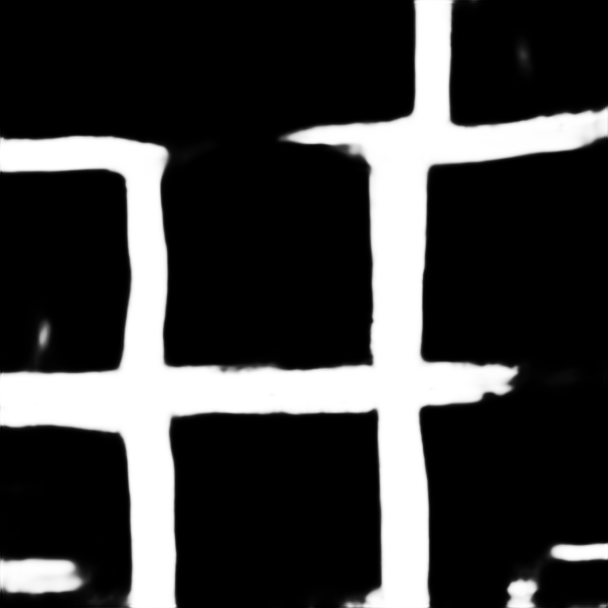
\includegraphics[width=0.4\linewidth]{fcn.png} \\
    \end{tabular}
    \caption{Top left original image. Top right baseline prediction. Bottom left better baseline prediction. Bottom right FCN prediction.}
    \label{fig:results}
\end{figure}

The baseline CNN model is by far the worst model for this task. The $16 \times 16$ patches used with this architecture contain far too little information to make an educated guess. This is true even for the trained human eye. In \autoref{fig:results} its clear that this model suffers from an abundance of false positives and false negatives.

Using $64 \times 64$ patches as we did in our second baseline model helped a tremendous amount. The larger patch size provides the model more context. Post-processing the input, whether with an SVN or a CNN helped but not significantly. We noticed that improvements of the initial predicting model impacted the performance of the post-processing model, but not vice-versa. In \autoref{fig:results} the results are slightly better than the baseline model. There is more structure to the data and less false positives. However, there are big structural gaps and a large amount of false negatives.

Fully convolutional architectures proved to be much more powerful than traditional CNN approaches. Even though we are not directly optimizing patch label prediction, better per pixel label prediction led to a better patch label prediction. As for the network type, Unet or FCN, we see very similar results at the high end and further data is needed to make a thorough comparison. The results of this model are shown in \autoref{fig:results}.

Pre-trained networks on much bigger datasets, such as ImageNet, significantly improved performance. These networks allowed us to use much deeper architectures, like the 101 layer ResNet, which would have been impossible to train with our tiny dataset.
